\chapter{Pair Localization Transition}

Natural first question: Does this system exhibit a localization transition (as captured by the standard indicators) and what are the conserved quantities.

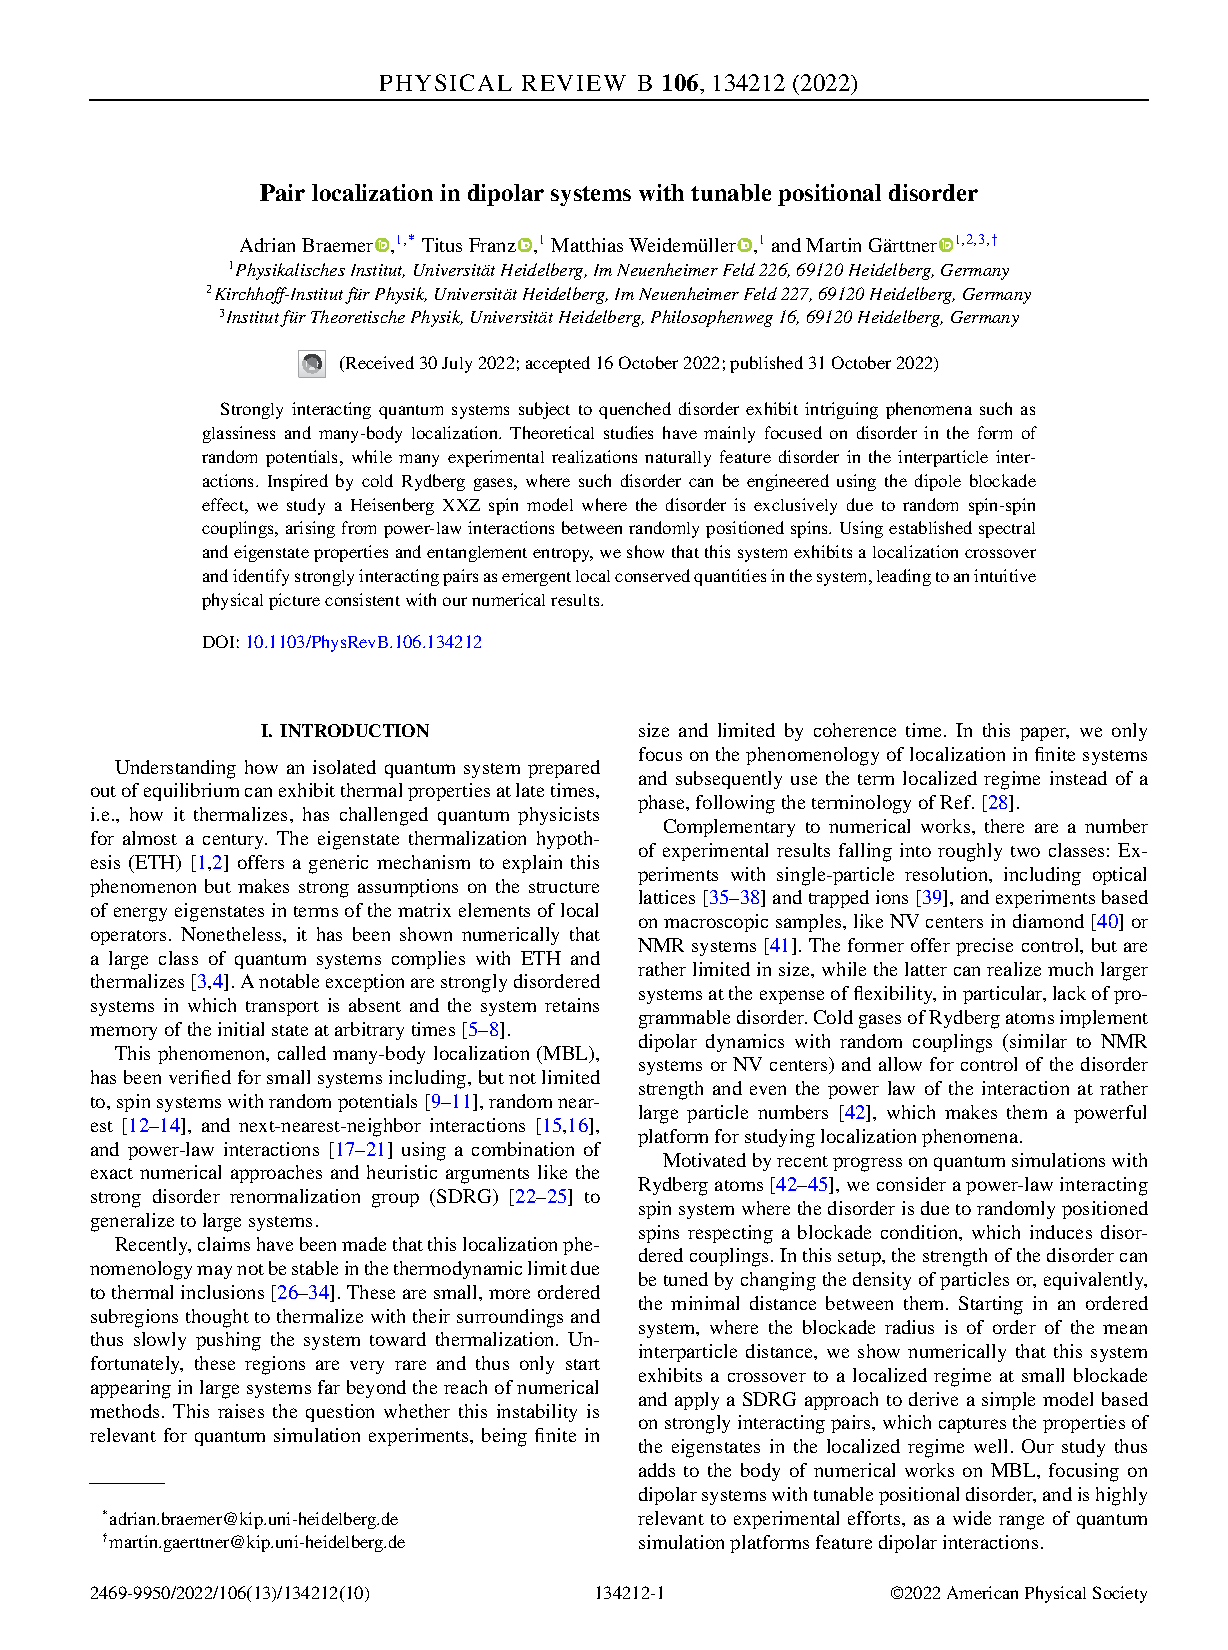
\includepdf[pages=-]{pub-Braemer2022-Pairlocalization}

\chapter{Efficient Numerics with Cluster Truncated Wigner Approximation}

can we exploit the knowledge about the conserved quantities to make numerics more efficient?

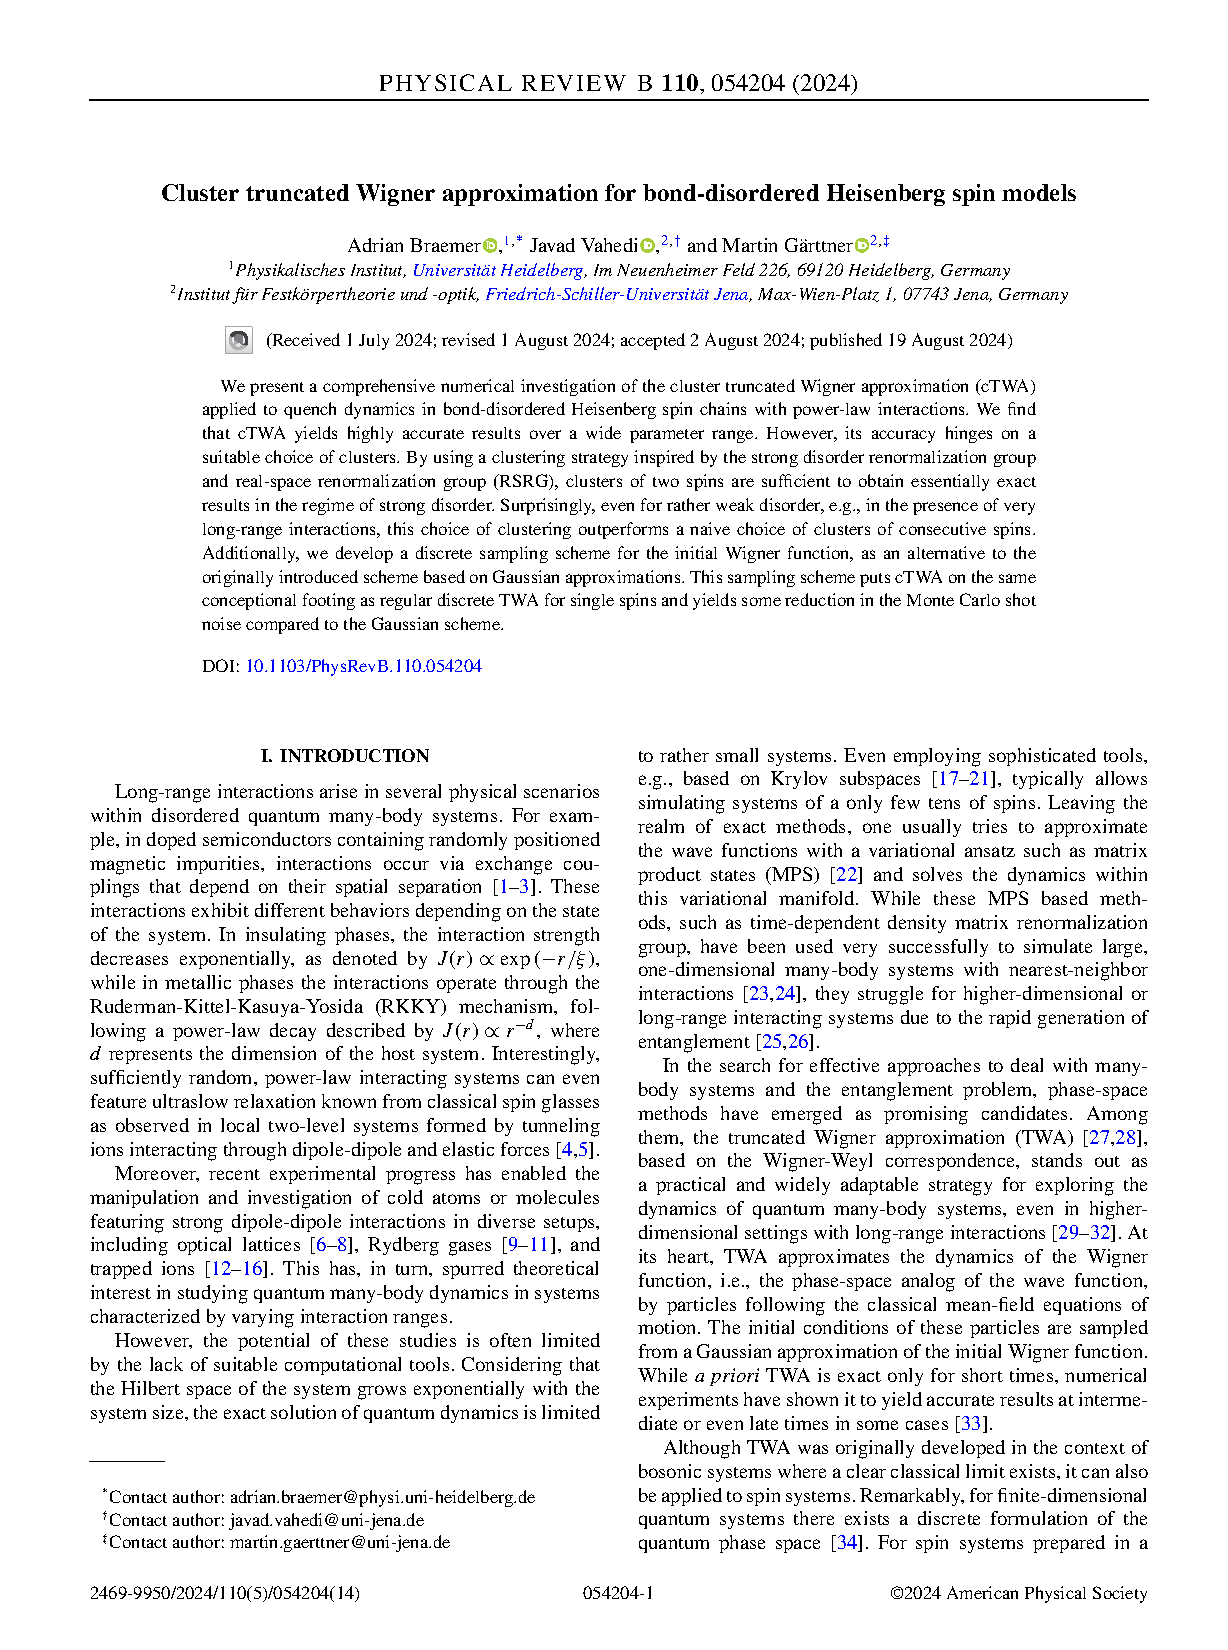
\includepdf[pages=-]{pub-Braemer2024-cTWA}